% !TEX encoding = UTF-8
% !TEX TS-program = pdflatex
% !TEX root = ../tesi.tex

%**************************************************************
\chapter{AWS EC2 resources generation with Pulumi}
\label{cap:case-study}
%**************************************************************

\intro{The implementation of a TypeScript solution and a Scala solution of a case study are here presented. Following, we have the implementation of the Scala syntactic sugar created for supporting Pulumi and how I managed to automate its generation}\\

%**************************************************************
\section{Amazon Web Services}
AWS is a wide collection of services with many different purposes and characteristics including computation, storage, databases, analytics, networking, mobile, developer tools, management tools, IoT, security, and enterprise applications.
All these services are on-demand, available in seconds, with pay-as-you-go pricing.
Anyway, for the purpose of the thesis we'll focus only on the EC2 module.

\subsection{AWS's EC2 module}
EC2 (Elastic Computing 2) provides scalable computing capacity in the Amazon Web Services (AWS) Cloud.
Amazon EC2 eliminates the need to invest in hardware up front, so that the development and deployment of the applications is faster.\\
It includes networking tools, container services, tools to manage scalability, and more.


\section{Case study infrastructure overview}
For the thesis, only few components of the vast EC2 module have been selected to create a working infrastructure.

\subsection{Components of the infrastructure}
The infrastructure I created for the case study of the thesis is an AWS EC2 \gls{VPC} hosting 3 private \gls{subnet}s, 3 public subnets, an \gls{internet gateway} to let the public subnets connect to the internet and a \gls{routing table} to map the public subnets to the internet gateway.
The architecture looks like this:
\begin{center}
  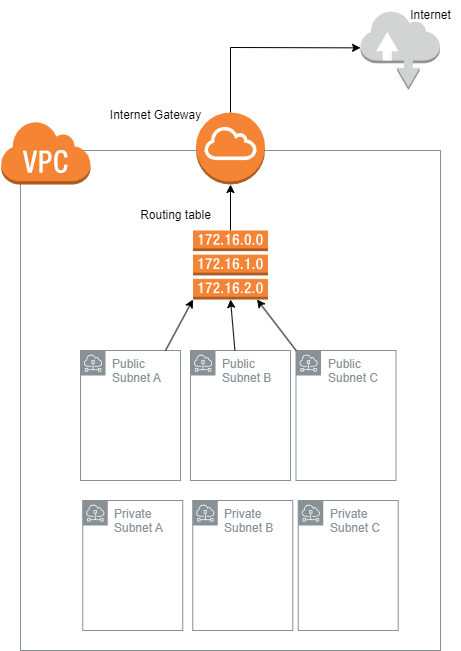
\includegraphics[width=1\columnwidth]{case_study/vpc_diagram} 
  \captionof{figure}{Infrastrutcture Architecture}
\end{center}\mbox{}\\
AWS is divided into regions, like us-east-1, eu-central-1, eu-south-1, etc.
For the purpose of our thesis eu-south-1 as a region has been chosen.
The servers of such a region are located in Milan.
Each region can have multiple availability zones, eu-south-1 has 3 different availability zones, and because of this I chose to create 3 couples of public/private subnets (A-A, B-B, C-C).
One couple on each availability zone.
The purpose of the availability zones is mainly for robustness.
If an availability zone becomes temporary unavailable, we can rely on the others to keep our services up.


\subsubsection{VPC}
The VPC is our "container" for all the other infrastructure resources.
We'll define the subnets, the internet gateway, and the routing table within such a VPC.\\
The most important setting of our AWS EC2 VPC is the CIDR (Classless Inter-Domain Routing) block.
It represents the range of private IP addresses that the VPC can use to create and manage resources within the VPC.
\paragraph{CIDR}
The CIDR block is used to define the range of IP addresses that the VPC can use.
In our case the CIDR block is 10.136.0.0/24, which means that the VPC has access to all IP addresses from 10.136.0.0 to 10.136.0.255.
The 24 in the CIDR block is the prefix length, aka the subnet mask, that is used to identify the VPC.
The remaining 8 bits of the IP address will be used to identify the hosts in the VPC.\\
We'll assign a name as well to our VPC so that will be easier to recognize it when we'll inspect the AWS Management Console, that is the GUI version of the AWS CLI.

%val pvtSubnetsCidrs: List[String] = List("10.136.0.0/27", "10.136.0.32/27", "10.136.0.64/27")
%val pubSubnetsCidrs: List[String] = List("10.136.0.96/27", "10.136.0.128/27", "10.136.0.160/27")

\subsubsection{Subnet}
The subnets will require the ID of the VPC and the CIDR block that defines their IP scope.
For the subnets we'll use the following CIDR blocks:
\begin{itemize}
  \item Private Subnet A: 10.136.0.0/27
  \item Private Subnet B: 10.136.0.32/27
  \item Private Subnet C: 10.136.0.64/27
  \item Public Subnet A: 10.136.0.96/27
  \item Public Subnet B: 10.136.0.128/27
  \item Public Subnet C: 10.136.0.160/27
\end{itemize}
3 of the 8 bits left out for the hosts identification have been used to identify the subnets.
In fact we shall notice that now the subnet mask is not 24 anymore, but 27.
Hence, we are left with 5 bits to identify the hosts within each subnet, giving us 32 possible IPs.
From such IPs 2 are reserved for the network address and the broadcast address, so we have 30 possible IPs.
We won't discuss this topic any further since it isn't essential for the final objective of the thesis.\\
Moreover, we'll define also the availability zone for each subnet.


\subsubsection{InternetGateway}
The definition of the internet gateway is actually quite straight forward.
The mandatory parameter to assign is the ID of the VPC.

\subsubsection{RouteTable}
\label{sssec:routetable}
The definition of a route table is required in order to bind the public subnets to the internet gateway, so that they can send and receive data over the internet.\\
Here, along with the VPC ID, we assign the routes of such routing table.
In order to do this we have to provide a CIDR and a target resource to which the packet will be forwarded to, that can be a subnet or the internet gateway in our case.
The internet gateway is mapped with the CIDR block 0.0.0.0/0.
Obviously also the ID of the internet gateway is required in order to bind it to the routing table.\\
In a nutshell this means that every packet not directed to a host within the VPC will be routed to the internet gateway and then to the internet.\\
The association of the public subnets to the routing table will be achieved using the \textit{route table association} resource.
Such a resource will require us to provide the ID of the subnet and the ID of the routing table to establish a connection.
The private subnets will not be associated to such a routing table, since we want to keep them private.
In fact, without explicitly associating them to a given routing table, AWS will automatically associate them to a default routing table that, being not bound to an internet gateway, will keep them private.\\


\section{TypeScript implementation of the case study}
\label{sec:typescript-impl}
The first version of the implementation of the previously defined architecture is written using the TypeScript APIs of Pulumi.
The structure of the project, and this holds for the Scala version as well, is trivial.
We have a simple \texttt{index.ts} file that defines the entry point for our TypeScript project, and it is just a couple of lines long:\\
\begin{minipage}{\linewidth}
\begin{lstlisting}[numbers=left, numberstyle=\tiny, numbersep=-5pt, stepnumber=1]
    import { VPC } from './VPC/VPC';
  
    const vpc = new MyVPC("Custom VPC");
  \end{lstlisting}
\end{minipage}
The interesting part relies on the \texttt{MyVPC} class.
Such a class extends the \texttt{ComponentResource} class of Pulumi.
In our TypeScript implementation, we use the constructor of the user-defined \texttt{MyVPC} class to call all its class methods, that are responsible for the creation of the resources.
We won't discuss this section further since the interesting part of the code are the actual methods that are responsible for the creation of the resources.

\subsection{VPC resource creation}
The call to the VPC resource creation API of Pulumi is done in this method of the \texttt{MyVPC} class:\\
\begin{minipage}{\linewidth}
\begin{lstlisting}[language=scala, numbers=left, numberstyle=\tiny, numbersep=-5pt, stepnumber=1]
  protected createVPC() {
    this.vpc = new Vpc("vpc_res", {
      cidrBlock: "10.136.0.0/24",
      tags: {Name: "myVPC-typescript"},
    },
    {
      parent: this,
    });
  }
\end{lstlisting}
\end{minipage}
\texttt{vpc\_res} is the name that will be given by Pulumi at this resource once on the \textit{stack}.
We can notice how the various parameters are given in a declarative style within the curly brackets.
Such a syntax is \textit{syntactic sugar} for a \texttt{Map} definition.\\
At line 9 the parent of this resource is set.
With this specification, we are telling to the \textit{stack} of Pulumi that the VPC resource \texttt{vpc\_res} that we are creating is a child resource of the resource identified by the \texttt{MyVPC} class, that in practice is nothing but a container for the other resources.

\subsection{Internet gateway creation}
To create the internet gateway resource we can use the following code:\\
\begin{minipage}{\linewidth}
\begin{lstlisting}[numbers=left, numberstyle=\tiny, numbersep=-5pt, stepnumber=1]
  protected createIGW(){
    this.gw = new InternetGateway("gw", {
      vpcId: this.vpc?.id,
      tags: {
          Name: "myIGW-typescript",
      },
    },
    {
      parent: this.vpc,
    });
  }
\end{lstlisting}
\end{minipage}
It is really simple since it requires just the ID of the VPC in which it has to be created and optionally a name and a parent for the Pulumi's \textit{stack} representation.


\subsection{Subnets creation}
To create the private and the public subnets we require a more complex logic.
The function that has been used is \texttt{protected createAZsSubnets(isPvt: Boolean)}.
It is called twice, once with a \texttt{true} value to create the private subnets, and another one with \texttt{false} to instantiate the public ones (and connect them to the routing table bound with the internet gateway).\\
In the body of the function, first we want to get all the availability zones present in the AWS region we are working on.
To achieve this, we will use such a function \texttt{this.availableZones = aws.getAvailabilityZonesOutput()}.\\
Second, we want to create both a private and public subnet in each availability zone acquired with the aforementioned method.
The \texttt{pulumi.all} function, in combination with the \texttt{apply} function will help us in achieving such a goal.\\

\subsubsection{pulumi.all}
\label{sssec:pulumi-all}
\texttt{pulumi.all} is a utility function in Pulumi that allows you to combine multiple \texttt{Output}s into a single \texttt{Output}.
So if we consider the following code:\\
\begin{minipage}{\linewidth}
\begin{lstlisting}[numbers=left, numberstyle=\tiny, numbersep=-5pt, stepnumber=1]
  pulumi.all([this.availableZones.names, this.vpc!.id])
\end{lstlisting}
\end{minipage}
Such a call returns us an \texttt{Output<[string[], string]>}.
The array of strings is the list of the availability zones names, while the second string represents the ID of our VPC on AWS EC2.
Now we have a new \texttt{Output} type that is more suitable to create the subnets based on our VPC ID, because the function apply is letting us "open" an \texttt{Output} value and access its content.

\subsubsection{.apply}
Let's extend our code in this way:\\
\begin{minipage}{\linewidth}
\begin{lstlisting}[numbers=left, numberstyle=\tiny, numbersep=-5pt, stepnumber=1]
  pulumi.all([this.availableZones.names, this.vpc!.id]).apply(([azNames, vpcId]) => {
    // lambda's body to create the subnets here
  })
\end{lstlisting}
\end{minipage}
The apply function is letting us access \texttt{Output<[string[], string]>} and apply some logic on the inner values.\\

\paragraph{The apply's lambda}
\label{par:ts-lambda}
Now that we have the access to the list of availability zones and the VPC ID, we can iterate over the availability zones and create the subnets for our VPC.
Here is the complete code of the function:\\
\begin{minipage}{\linewidth}
\begin{lstlisting}[numbers=left, numberstyle=\tiny, numbersep=-5pt, stepnumber=1]
  protected createAZsSubnets(isPvt: Boolean) : Output<Subnet[]>{
    this.availableZones = aws.getAvailabilityZonesOutput()
    return pulumi.all([this.availableZones.names, this.vpc!.id]).apply(([azNames, vpcId]) => {
      let i = 0
      let listToPushInto: Subnet[] = Array<aws.ec2.Subnet>()
      azNames.forEach(azName => {
        let fullName = azName + (isPvt ? "-pvt" : "-pub") + "-subnet-typescript"
        listToPushInto.push(new Subnet(fullName, {
          vpcId: vpcId,
          availabilityZone: azName,
          cidrBlock: isPvt ? this.pvtSubnetsCidrs[i] : this.pubSubnetsCidrs[i],
          tags: {
            Name: fullName,
          },
        },{
          parent: this.vpc
        }));
        i++;
      });
      return listToPushInto
    });
  }
\end{lstlisting}
\end{minipage}
In the code we instantiate private or public public subnets basing on the \texttt{isPvt} passed in the \texttt{createAZsSubnets}.
We can notice that for the creation of a subnet we pass arguments such as \texttt{vpcId}, the availability zone name, the CIDR block, and a name (that is a tag) to better identify it on the \textit{stack}.\\
Each newly created subnet is then pushed into the class field \texttt{this.prvSubNets} or \texttt{this.pubSubNets} (that are arrays of subnets), basing on the nature of the subnet.\\
The creation of a subnet requires us to provide both the availability zone name and the ID of the VPC.
Since these two pieces of information are contained in two separate \texttt{Output}s (\texttt{Output<String[]>} and \texttt{Output<String>} respectively) we must first use the \texttt{pulumi.all} to wrap them in a single \texttt{Output<String[], String>}.
This due to the fact that \texttt{.apply} can accept a single \texttt{Output<A>}, for any \texttt{A} type, value as input and not a pair.
Then, we can use the \texttt{.apply} to \textit{unbox} from the \texttt{Output<String[], String>} its inner value.
Now that we have both the pieces of information out of the \textit{context} value, we can use them to create the subnets.\\
%The \texttt{this.pubSubNets} will be used by the \texttt{this.attachRouteTableToPubSubnets()} function to bind the public subnets to the internet gateway through the routing table.\\
%The crucial point here is that in order to bind the public subnets to the routing table, we must call \texttt{this.attachRouteTableToPubSubnets()} as the last step in our \texttt{pulumi.all} function call.
%This ensures that we have all the necessary subnets to make the binding, since the call will be done at the completion of the creation of the subnets.
We can notice that the \texttt{.apply} function is, at the end of its lambda, returning a list of the created subnets.
Since the \texttt{apply} function wraps any returned value inside an \texttt{Output} \textit{context}, its actual return type is \texttt{Output<Subnet[]>}.
Such a return value is also the whole functions's one.

\subsection{Routing table creation}
This is the code to create the routing table resource:\\
\begin{minipage}{\linewidth}
\begin{lstlisting}[numbers=left, numberstyle=\tiny, numbersep=-5pt, stepnumber=1]
  protected createRouteTable() {
    this.routeTable = new RouteTable("example", {
      vpcId: this.vpc!.id,
      routes: [
          {
              cidrBlock: "0.0.0.0/0",
              gatewayId: this.gw!.id,
          },
      ],
      tags: {
          Name: "myRouteTable-typescript",
      },
    },
    {
      parent: this.vpc,
    });
  }
\end{lstlisting}
\end{minipage}
On top of the classic VPC ID we are assigning here the routes.
As we mentioned before in the \hyperref[sssec:routetable]{Routetable} paragraph, we are defining the route with CIDR 0.0.0.0/0 to redirect all the packets coming from the public subnets, and not having as destination an IP internal to our VPC, to the internet gateway.\\
We are also giving a name to the routing table and assigning its parent.


\subsection{Attaching the public subnets to the internet gateway}
As we mentioned previously, we use the \texttt{this.attachRouteTableToPubSubnets()} function to attach the public subnets to the internet gateway.
Here is the code of the function:\\
\begin{minipage}{\linewidth}
\begin{lstlisting}[numbers=left, numberstyle=\tiny, numbersep=-5pt, stepnumber=1]
  protected attachRouteTableToPubSubnets(){
    let i = 0
    this.pubSubNets.apply(subNets => {
      subNets.forEach(sn => {
        new aws.ec2.RouteTableAssociation(`${i}-routeTableAssociation-typescript`, {
          subnetId: sn.id,
          routeTableId: this.routeTable!.id,
        },
        {
          parent: this.vpc
        });
        i++
      })
    });
  }
\end{lstlisting}
\end{minipage}
Here we used once more, as for the subnets creation, a combination of \texttt{apply} and the \texttt{foreach} to iterate over all the subnets "\textit{unboxed}" from the \texttt{Output} \textit{context}.
Also here, we \textit{unbox} the \texttt{Subnet[]} value from the \texttt{Output} with the aid of the \texttt{apply} function, and then we iterate over the subnet array with the \texttt{foreach}.\\
Inside the \texttt{foreach}'s lambda we are defining a new \texttt{RouteTableAssociation} AWS EC2 resource that requires just the ID of the subnet and the ID of the routing table to which we want to attach the subnet to.

\section{Creating the resources with Pulumi}
\label{sec:ts-res-creation}
After having seen all the code to create the resources, we'll see what the Pulumi command \texttt{pulumi up} will do.
The command checks if all the resources that we want to create have valid parameters and there are not circular dependencies among the resources on their creation.
If everything is nice and neat, it will shows us the preview of the changes that we are about to get:
\begin{center}
  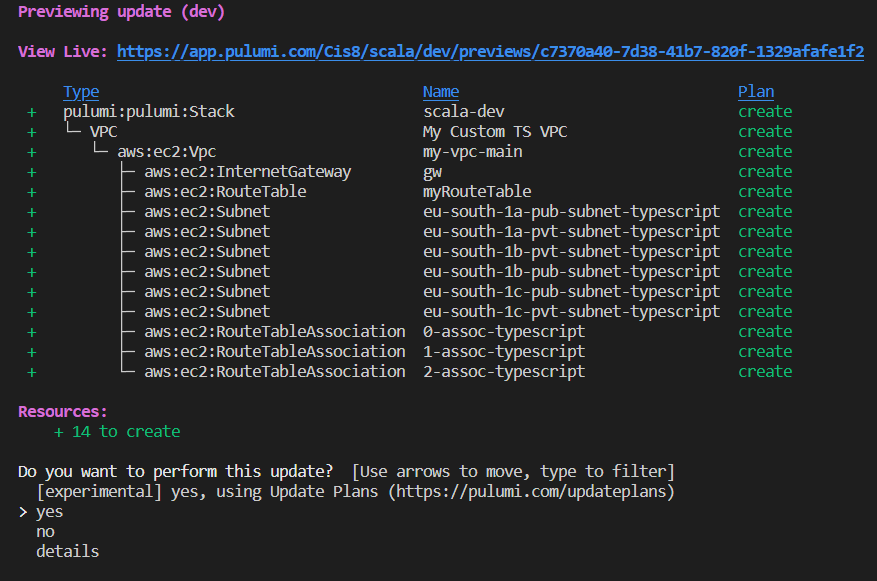
\includegraphics[width=1\columnwidth]{case_study/pulumi_up_1} 
  \captionof{figure}{pulumi up preview}
\end{center}\mbox{}\\

If we press yes this is the output:
\begin{center}
  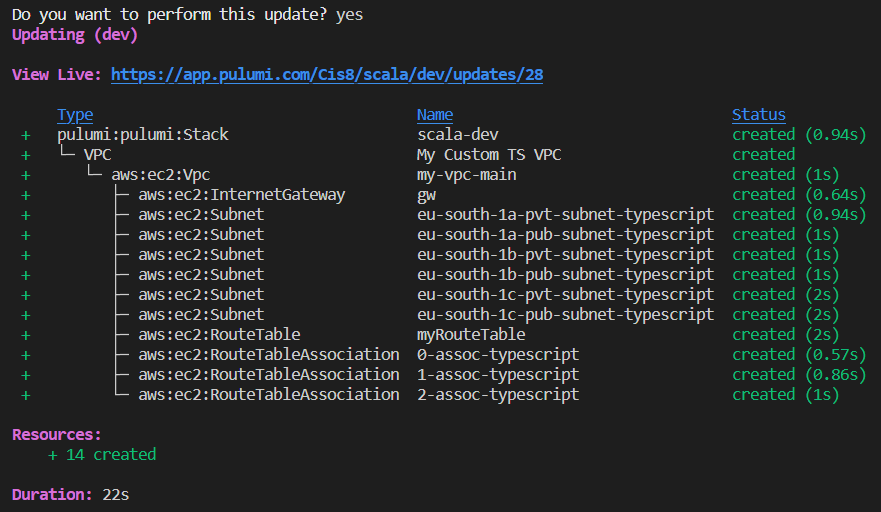
\includegraphics[width=1\columnwidth]{case_study/pulumi_up_2} 
  \captionof{figure}{pulumi up confirmed}
\end{center}\mbox{}\\
We can notice how the resources created are nested into each other thanks to the parent option that we used.
This is helping us in keeping our resources on the \textit{stack} nicely ordered and tied up.
Moreover, we can notice how they are neatly nested thanks to the usage of the \texttt{parent} extra option.\\

\section{Destroying the resources with Pulumi}
Now let's use the \texttt{pulumi destroy} command to destroy the resources on our Pulumi's \textit{stack}.
The preview of the changes that we are about to get looks like this:
\begin{center}
  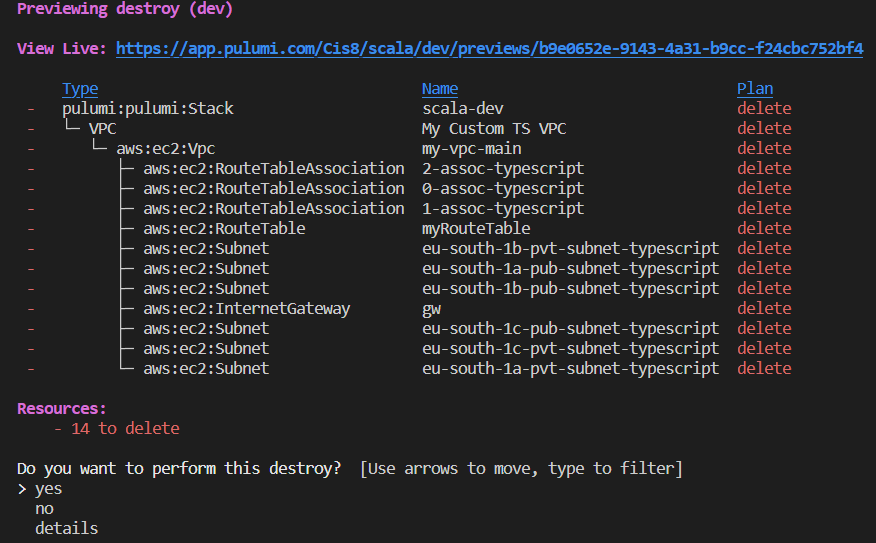
\includegraphics[width=1\columnwidth]{case_study/pulumi_destroy_1} 
  \captionof{figure}{pulumi destroy preview}
\end{center}\mbox{}\\

If we confirm the changes this is the result:
\begin{center}
  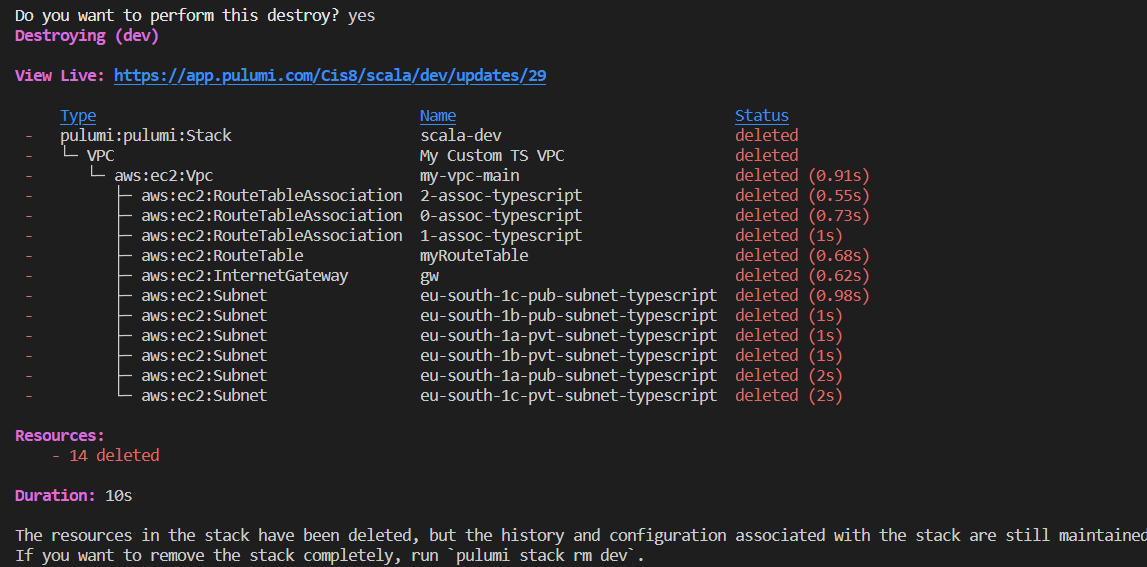
\includegraphics[width=1\columnwidth]{case_study/pulumi_destroy_2} 
  \captionof{figure}{pulumi destroy confirmed}
\end{center}\mbox{}\\

%\section{Java implementation of the case study}

\section{My Scala implementation of the case study}
Since Scala is not supported by Pulumi, I had to get around this somehow.
As I mentioned in the \hyperref[sssec:off-support-pulumi]{The onerous work to officially support a new language in Pulumi} section, an official support of Scala for Pulumi was unfeasible, hence a custom and partial support of Scala has been achieved.
The idea behind the adopted solution is to exploit the compatibility of Scala with the Java libraries to write custom \textit{syntactic sugar}.
Such \textit{syntactic sugar} will be based on the Pulumi Java's APIs and will provide to the user cool constructs to write readable and expressive code to interact with Pulumi.\\
The steps of the work done have been the followings:
\begin{enumerate}
  \item manually write the \textit{sugared} Pulumi API functions to create the Pulumi resources using Scala
  \item use such APIs to recreate the \textit{stack} obtained with the TypeScript solution shown before in the \hyperref[sec:ts-res-creation]{Creating the resources with Pulumi} section
  \item create an automatic code generator for our \textit{syntactic sugar} functions, so that we can quickly create a library for Scala's Pulumi APIs
  %\item try to recreate the \textit{stack} with the automatically generated code
\end{enumerate}
Obviously, the third step is quite wide, and if fact with my work I had generated only the functions for a part of the Scala's Pulumi APIs for the AWS EC2 module.\\
The just defined steps will be now more accurately presented.

\subsection{Structure of the Java APIs for the constructors of the resources in Pulumi}
To understand the \textit{syntactic sugar} functions that I defined, let's first consider the general structure of the Java APIs for the constructors of the resources.\\
The constructor of a resource, in general accepts a name and an instance of the corresponding \texttt{Args} class of the resource we are creating.
Let's consider for example the Vpc resource.
In Java, to instantiate such a resource we'd call:\\
\begin{minipage}{\linewidth}
\begin{lstlisting}[numbers=left, numberstyle=\tiny, numbersep=-5pt, stepnumber=1]
  protected Vpc vpc = new Vpc("my-vpc-java", VpcArgs.builder()
    .cidrBlock("10.136.0.0/24")
    .tags(Map.of("Name", "main"))
    .build(),
          CustomResourceOptions.builder()
                  .parent(this)
                  .build());
\end{lstlisting}
\end{minipage}
We can see that along with the name to be assigned to the VPC "my-vpc-java", a \texttt{VpcArgs} builder and a \texttt{CustomResourceOptions} builder are passed by.
These builders will create an instance of the respective classes that will be used to set respectively the parameters and the parent of the \texttt{Vpc} resource.
So, for our case study we need to consider: the name to be assigned to the created resource on the Pulumi \textit{stack}, the builder of the respective \texttt{Args} class of the resource, and the \texttt{CustomResourceOptions} builder.


\subsection{\textit{syntactic sugar} usage}
\label{ssec:syn-sug-usage}
Our \textit{syntactic sugar} is split in 2 categories of functions.
The first is about the functions that represent the constructors of the resources.
The second is for the methods available within the builders of the \texttt{Args} classes and for the \texttt{CustomResourceOptions} builder's functions.
The idea to create a resource is to call the \textit{sugared} function that represent the constructor of that resource, and then call the \texttt{Builder}'s methods to assign the various parameters to the resource.

\subsubsection{Vpc creation}
\label{sssec:vpc-creation-scala}
This is how a Vpc resource can be created with my \textit{syntactic sugar}:\\
\begin{minipage}{\linewidth}
\begin{lstlisting}[numbers=left, numberstyle=\tiny, numbersep=-5pt, stepnumber=1]
  val myVpc = vpc("scala-main") ({
    cidrBlock("10.136.0.0/24")
    tags("Name" -> "myVpcScala")
  },{
    parent(this)
  })
\end{lstlisting}
\end{minipage}
At line 1, the \texttt{vpc} function is the actual \textit{sugared} function for the VPC resource constructor.
We can notice that we have a curried function.
The first parentheses are taking the parameter for the resource name on the Pulumi \textit{stack}, while the second ones contain two lambdas (defined by the curly brackets).
These lambdas are respectively used to call all the builder methods of the \texttt{VcpArgs} class and the \texttt{CustomResourceOptions}'s ones.\\
We can notice that we didn't explicitly define an instance of the builders of such classes.
We will soon see how we achieved such a \textit{syntactic sugar} trick.\\
\texttt{cidrBlock} and \texttt{tags} are the generated methods are the generated methods for the builder of the \texttt{VpcArgs} class.\\ 
\texttt{parent} is instead the generated method for the builder of the \texttt{CustomResourceOptions} class.\\
Moreover, we can also notice that inside tags, that expects a \texttt{Map[String, String]} type, the explicit call to the \texttt{Map} builder for the instantiation of a \texttt{Map[String, String]} containing a single element isn't required.
This other trick will be explained later as well.

\subsubsection{Internet gateway creation}
Much similar to the VPC resource, we have this code for the internet gateway creation:\\
\begin{minipage}{\linewidth}
\begin{lstlisting}[numbers=left, numberstyle=\tiny, numbersep=-5pt, stepnumber=1]
  val myIGW = internetGateway("gw") ({
    vpcId(myVpc.getId())
    tags("Name" -> "myIGWScala")
  },{
    parent(myVpc)
  })
\end{lstlisting}
\end{minipage}
The code won't be commented since is analogous to the VPC case.

\subsubsection{Routing table creation}
\label{sssec:routetable-creation-scala}
The code to create a routing table:\\
\begin{minipage}{\linewidth}
\begin{lstlisting}[numbers=left, numberstyle=\tiny, numbersep=-5pt, stepnumber=1]
  val myRouteTable = routeTable("myRouteTable") ({
    vpcId(myVpc.getId())
    routes(
      routeTableRouteArgs(){
        cidrBlock("0.0.0.0/0")
        gatewayId(myIGW.getId())
      })
    tags("Name" -> "myRouteTableScala")
  },{
    parent(myVpc)
  })
\end{lstlisting}
\end{minipage}
The only thing that is worth to mention here is that the \texttt{routes} function, at line 3, expects a \texttt{List[RouteTableRouteArgs]}, but we are providing only a \texttt{RouteTableRouteArgs}.
As for the case of the \texttt{Map[String, String]} with the \texttt{parent} method mentioned above, the same trick has been used to provide the \textit{syntactic sugar} that lifts us from the need of instantiate a singleton \texttt{List[RouteTableRouteArgs]} manually.

\subsubsection{Subnets creation}
\label{sssec:subnets-creation}
Much different from the other resources is the function to create the subnets:\\
\begin{minipage}{\linewidth}
\begin{lstlisting}[numbers=left, numberstyle=\tiny, numbersep=-5pt, stepnumber=1,linewidth=420pt]
  def createAzSubnets(isPvt: Boolean) =
      for
        azRes <- availabilityZonesNames()
        myVpcId <- myVpc.id()
        tuples = azRes.names().zip(if isPvt then pvtSubnetsCidrs else pubSubnetsCidrs)
      yield
        tuples.map((name, cidr) => {
          val fullName = name + "-" + (if isPvt then "pvt" else "pub") + "-subnet-scala"
          subnet(fullName) ({
            vpcId(myVpcId)
            availabilityZone(name)
            cidrBlock(cidr)
            tags("Name" -> fullName)
          },{
            parent(myVpc)
          })
      })
\end{lstlisting}
\end{minipage}
We can notice how we achieved to get a solution that is relying only on the for yield construct thanks to the monad for the \texttt{Output} type, that we will soon see how it is actually implemented.\\
The \texttt{azRes} enumerator is extracting a \texttt{GetAvailabilityZonesResult} object out from the \texttt{Output[GetAvailabilityZonesResult]} object returned by \texttt{availabilityZonesNames()}. 
Similarly, the \texttt{myVpcId} enumerator is instead extracting the ID of the VPC from the \texttt{Output[String]} value coming from \texttt{myVpc.id()}.
\textbf{These two enumerators are the replacement of the} \texttt{pulumi.all} \textbf{function in the TypeScript solution.}
These extractions are possible only thanks to the mondadic implementation of the \texttt{Otput} type. 
In fact this \textit{syntactic sugar} of the for yield is, behind the scenes, implemented as a concatenation of the \texttt{map} and \texttt{flatMap} functions.
So, the fact that our for yield is able to work on \texttt{Output} types is possible only because of the monadic implementation of the \texttt{Output} type that is exposing the \texttt{map} and \texttt{flatMap} methods to be used by the for yield behind the scenes.\\
%The fact that these functions are by the \texttt{Monad[Output]} type, we can use our for yield to work on \texttt{Output} types.\\
At line 4 we have the definition of the \texttt{tuple} value as a zipping of the availability zone names (extracted with the \texttt{.names()} function) and the respective CIDR blocks.
The tuples are mapped with a lambda that declares the various subnets to be created.
Now, the yield is concatenating the various declared subnets in a single \texttt{Output[Iterable[Subnet]]}, that is the return type of the for yield and of the whole function.\\
%Finally, we should observe that the for yield takes an \texttt{Output[A]} (the enumerators) and returns an \texttt{Output[B]}, where \texttt{A = GetAvailabilityZonesResult} and \texttt{B = Output[Iterable[Subnet]]}, that is resembling to the \texttt{map} and \texttt{flatMap}'s input/output types.
%These are the exact input/output types granted from the map and flatMap functions declared in the \texttt{Monad[Output]} as we will see soon.


%We can notice here how we had the possibility to use the \texttt{map} function on \texttt{availabilityZonesNames()}.
%\texttt{availabilityZonesNames()} returns a \texttt{Output[GetAvailabilityZonesResult]} value, that isn't directly accessible from the \texttt{map} function.
%To achieve such a result we made a monad out of the \texttt{Output} type, so that map can be applied on the inner value of the \texttt{Output} \textit{context}.
%We'll see better how is the actual implementation of the monad soon.\\
%The for yield construct here is iterating over a zipped list made out of the availability zones names and the CIDR blocks for the respective kind of subnet to create (private or public, based on the input parameter isPvt).
%The for yield, for each tuple \texttt{(name, cidr)} will create a \texttt{Subnet} value and will return a \texttt{Subnet[]} as output.
%Now, the for is still inside the lambda of the \texttt{availabilityZonesNames().map} function.
%Consider the fact that \texttt{map} takes an \texttt{Output[A]} and returns an \texttt{Output[B]}, where \texttt{A = GetAvailabilityZonesResult} and \texttt{B = Output[Iterable[Subnet]]}.
%This is different from the TypeScript implementation in the \hyperref[par:ts-lambda]{Apply's lambda} paragraph, where the function that creates the subnets returns a plain \texttt{Subnet[]}.\\
%We will make further considerations about such a difference in the \hyperref[cap:comparisons]{Comparison between the languages for Pulumi and the advantages of Scala} chapter.\\

\subsubsection{Attaching the subnets to the routing table}
\begin{minipage}{\linewidth}
\begin{lstlisting}[numbers=left, numberstyle=\tiny, numbersep=-5pt, stepnumber=1]
  def attachRouteTableToPubSubnets() = // Output[Iterable[RouteTableAssociation]] 
        for
          subnets <- pubSubnets
          tuples = subnets.zipWithIndex
        yield
          tuples.map((ps, idx) => routeTableAssociation(idx + "-assoc-scala") ({
            subnetId(ps.getId())
            routeTableId(myRouteTable.getId())
          }, {
            parent(myVpc)
          }))
\end{lstlisting}
\end{minipage}
Similarly to the subnet creation function, also here we use the for enumerators to "\textit{unbox}" an \texttt{Output[Iterable[Subnet]]} value.
After having zipped the subnets to the indexes, whose only purpose is to give a custom name to the created associations, we iterate over the tuples to declare the associations with the aid of a \texttt{map} function.\\
Since the logic is analogous to the \texttt{createAzSubnets} function we won't comment this code further.
%The fact we're having these two functions that both take an \texttt{Output[A]} as input and return an \texttt{Output[B]} will be a key point for our observations in the \hyperref[cap:comparisons]{Comparison between the languages for Pulumi and the advantages of Scala} chapter.
%Similarly to the subnet creation function, also here we use map to "\textit{unbox}" an \texttt{Output[Iterable[Subnet]]} value, to apply some logic on the inner value and then return a \texttt{Output[Iterable[RouteTableAssociation]]} value as result.
%Since the logic is analogous we won't comment this code further, but the fact we're having these two functions that both take an Output[A] as input and return an Output[B] will be a key point for our observations in the \hyperref[cap:comparisons]{Comparison between the languages for Pulumi and the advantages of Scala} chapter.

\subsubsection{Resources creation with pulumi up}
\label{sssec:res-cre-ts}
Now let's make sure that the \textit{stack} created with \texttt{pulumi up} is the same of the one created with the TypeScript implementation.
From this image we can see that they are equivalent to the ones shown in \hyperref[sssec:res-cre-ts]{Resources creation with pulumi up in TypeScript}:
\begin{center}
  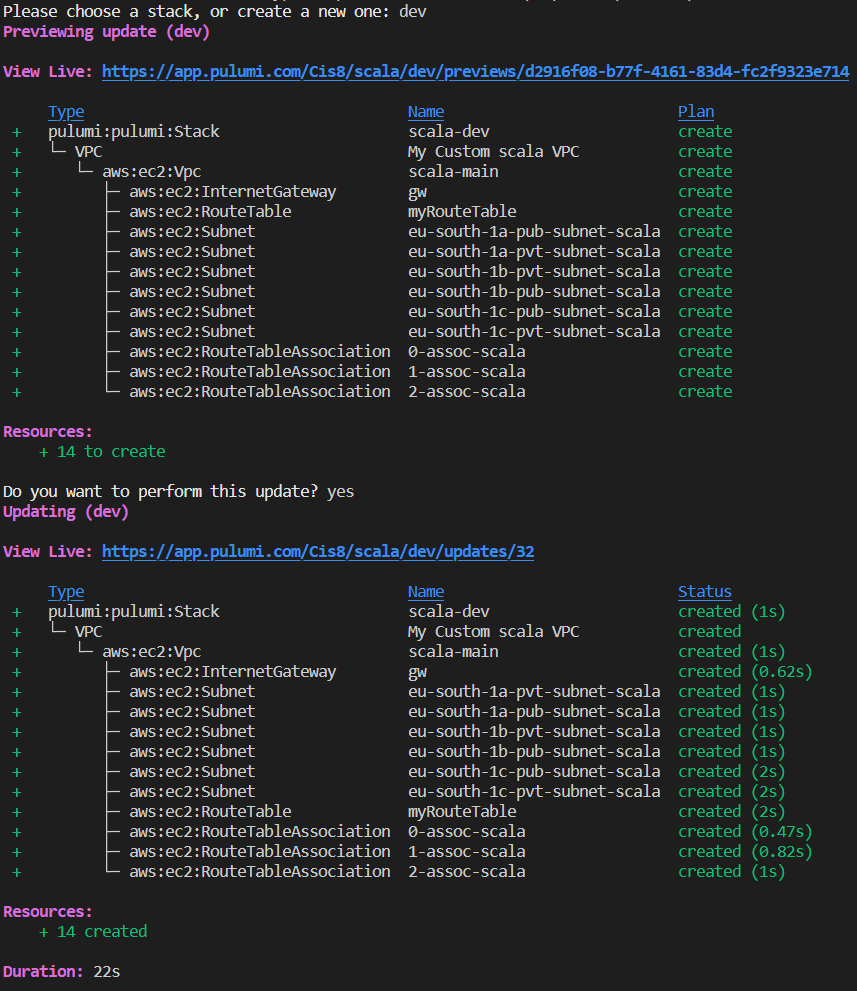
\includegraphics[width=1\columnwidth]{case_study/pulumi_up_scala_result} 
  \captionof{figure}{pulumi up result with the scala implementation}
\end{center}\mbox{}\\

\subsection{\textit{syntactic sugar} for the constructors of the resources}
All the methods that we just used for creating the Pulumi resources in Scala (\texttt{vpc, internetGateway}, etc.), behind the scenes are implemented following a common pattern.
Consider the \texttt{vpc} function of the \textit{syntactic sugar} defined inside the "PulumiUtilFunctionsForScala.scala" file:\\
\begin{minipage}{\linewidth}
\begin{lstlisting}[numbers=left, numberstyle=\tiny, numbersep=-5pt, stepnumber=1]
  def vpc(param: String)
         (init: VpcArgs.Builder ?=> Unit,
          initOpt: (CustomResourceOptions.Builder ?=> Unit) = baseOpts): Vpc =
	  given b: VpcArgs.Builder= VpcArgs.builder()
	  init
	  given bo: CustomResourceOptions.Builder = CustomResourceOptions.builder()
	  initOpt
	  new Vpc(param, b.build(), bo.build())
\end{lstlisting}
\end{minipage}
Let's analyze the function by steps.
First of all we can see that the function declaration is curried, we have 2 parentheses with different input parameters.\\
The first parentheses take simply a \texttt{String} parameter, that is used to set the name of the \texttt{Vpc} resource on the Pulumi \textit{stack}.\\
The second parentheses are taking two lambdas as parameters: a \texttt{VpcArgs.Builder ?=> Unit}  and a \texttt{CustomResourceOptions.Builder ?=> Unit} with default parameter \texttt{baseOpts}. We'll see in a moment what \texttt{baseOpts} is.\\
In Scala, a lambda that takes an \texttt{Int} and returns a \texttt{String} has this type notation: \texttt{Int => String}, so does that '\texttt{?}' in front of the '\texttt{=>}' mean?\\
Such '\texttt{?=>}' is denoting a \textit{context} function, that is a function with (only) \textit{context} parameters.
In the \hyperref[par:given-using]{given and using keywords} paragraph we introduced the \texttt{using} keyword.
Such '\texttt{?}' is quite analogous to a \texttt{using} keyword used to mark a function input parameter as an implicit parameter.
This is, in part, what let us call the builder methods like \texttt{cidrBlock("10.136.0.0/24")} and \texttt{tags("Name" -> "myVpcScala")} 
without having to call them on a specific builder instance (as shown in the code shown in the \hyperref[sssec:vpc-creation-scala]{Vpc creation in Scala} paragraph).
We will get the whole picture of this trick when we'll talk about the \textit{syntactic sugar} for the builders' methods in the \hyperref[ssec:syn-sug-builders]{\textit{syntactic sugar} for the builders' methods} paragraph.\\
To conclude, in the function body we have the instantiation of the builders for the \texttt{VpcArgs} and \texttt{CustomResourceOptions} classes as given context parameters.
The \texttt{init} and \texttt{initOpt} lambdas, thanks to the '\texttt{?=>}' notation, are expecting a compatible context parameter to be taken in input.
Such lambdas will set the parameters of the respective given builders.
The function ends with the call to the Pulumi's Java API for the declaration of a \texttt{Vpc} resource, passing in the name of the VPC and the instances of the \texttt{VpcArgs} and \texttt{CustomResourceOptions} classes built using the respective builders.

\subsubsection{Correspondence between the input parameters and the user defined code used to create the VPC}
To have a better idea to what these parameters refer in our VCP creation case, consider this image:
\begin{center}
  \hspace*{-1cm}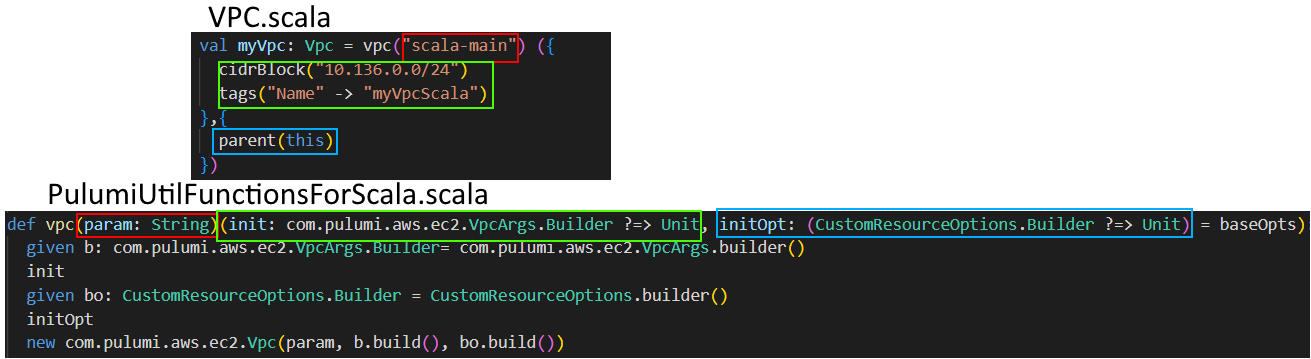
\includegraphics[width=1.3\columnwidth]{case_study/vpc_params_boxes} 
  \captionof{figure}{Parameters correspondence in the VPC declaration in Scala}
\end{center}\mbox{}\\
The red box represents the name for our VPC resource on the Pulumi \textit{stack}.\\
The green one, with the curly brackets, is the lambda that takes a \textit{given} \texttt{VpcArgs.Builder} as an implicit parameter from the \textit{context}.
In fact we are not providing any explicitly.
The \texttt{given b} defined in the first line of the body of the \texttt{vpc} function is the instantiation of a \textit{given} instance of such a builder, that will be automatically injected by the compiler in the \texttt{init} lambda represented by the green box.\\
Analogous is the concept for the blue box.\\

%\subsubsection{Vpc construction}
%Now that we understood what are the input parameters of our \texttt{vpc} function and to what do they correspond in the resource creation shown in the \hyperref[ssec:syn-sug-usage]{\textit{syntactic sugar} usage} section, we can see how the actual creation of the resource is made.
%After having executed the \texttt{init} and \texttt{initOpt} lambdas, that behind the scenes will set the parameters of the respective \textit{given} builders, we can create the resource using the constructor offered by the Pulumi Java APIs.
%\texttt{new Vpc(param, b.build(), bo.build())} is a direct call to such libraries, and will create actually create the \texttt{VPC}.

\subsubsection{The baseOpts function}
The \texttt{baseOpts} function that we mentioned before as a default lambda for our \texttt{vpc} function is the following:\\
\begin{minipage}{\linewidth}
\begin{lstlisting}[numbers=left, numberstyle=\tiny, numbersep=-5pt, stepnumber=1]
  def baseOpts(using o: CustomResourceOptions.Builder) : Unit = {}
\end{lstlisting}
\end{minipage}
In practice, it is a vacuous lambda that does nothing on the \texttt{CustomResourceOptions} builder.
The question here is: \textit{why do we need such a default function?}
To answer the question let's consider one more time the code to create a VPC with out \textit{syntactic sugar}:\\
\begin{minipage}{\linewidth}
\begin{lstlisting}[numbers=left, numberstyle=\tiny, numbersep=-5pt, stepnumber=1]
  val myVpc: Vpc = vpc("scala-main") ({
    cidrBlock("10.136.0.0/24")
    tags("Name" -> "myVpcScala")
  },{
    parent(this)
  })
\end{lstlisting}
\end{minipage}
We can see that we passed both the lambdas for the \texttt{VpcArgs} builder and for the \texttt{CustomResourceOptions} builder, but what if we want to simply use the \texttt{VpcArgs} builder and not set the parent?
We can do the following:\\
\begin{minipage}{\linewidth}
\begin{lstlisting}[numbers=left, numberstyle=\tiny, numbersep=-5pt, stepnumber=1]
  val myVpc: Vpc = vpc("scala-main") {
    cidrBlock("10.136.0.0/24")
    tags("Name" -> "myVpcScala")
  }
\end{lstlisting}
\end{minipage}
This code compiles, and we can notice that we even got rid of the parentheses around the curly brackets for the lambda.
If this compiles is only thanks to the default parameter that is automatically injected in by the compiler, as we didn't give an explicit one.\\
\newline
Another question might now arise: \textit{why didn't we change the signature of the function in the following way?}\\
\begin{minipage}{\linewidth}
\begin{lstlisting}[numbers=left, numberstyle=\tiny, numbersep=-5pt, stepnumber=1]
  def vpc(param: String)(using initOpt: (CustomResourceOptions.Builder ?=> Unit), init: VpcArgs.Builder ?=> Unit) : etc.
\end{lstlisting}
\end{minipage}
Here we have set the \texttt{initOpt} as an implicit parameter with the \texttt{using} keyword.
The main problems that we face with this solution are mainly two: we have to swap the order of the parameters and we will be forced to explicitly type the \textit{using} keyword if we want to pass custom lambda for the \texttt{CustomResourceOptions} builder.\\
The first problem leads to a sort of awkwardness while defining the VPC resource, since we have to define first the parent and then the actual parameters of the VPC resource.\\
%The second problem is a consequence of a Scala intrinsic characteristic, that requires us to explicitly write \texttt{using} when we want to explicitly pass an argument to a function's implicit parameter.\\
Moreover, these problems are due to the functioning of the Scala language.
An implicit parameter must come before all the explicit parameters and when trying to use an explicit parameter in place of an implicit one we must use the \texttt{using} keyword.
So, the original solution with the default parameter is the best one since it doesn't require us to swap the order of the parameters and we are totally free to choose whether to pass or not the explicit lambda for the \texttt{CustomResourceOptions} builder without worsening our \textit{syntactic sugar}.\\
Anyway, \textit{what if we modify the just presented alternative like this? Would it be better despite the fact that we would still require the} \texttt{using} \textit{keyword if we want to provide an explicit parameter?}\\
\begin{minipage}{\linewidth}
  \begin{lstlisting}[numbers=left, numberstyle=\tiny, numbersep=-5pt, stepnumber=1]
    def vpc(param: String)(init: VpcArgs.Builder ?=> Unit)(using initOpt: CustomResourceOptions.Builder ?=> Unit) : etc.
  \end{lstlisting}
\end{minipage}
Here we can notice that we set moved the implicit \texttt{initOpt} parameter in a new set of parentheses with the currying, granting us the chance to define first the VPC settings, and only then the custom options (i.e. setting the parent).
Anyway, we have a third problem that is affecting both this and the previous solution.
The implicit \texttt{initOpt} parameter requires us to provide a visible given instance for the implicit parameter in the site of call of the function.
In other words, leads to the awkward necessity to create, or import, a given instance of the \texttt{baseOpts} vacuous lambda in our VPC.scala file to have this solution work. 
Otherwise, the compiler would complain that there is no a given instance for the implicit parameter in scope.\\
With this extra constraint, the first proposed solution is, in my opinion, the one that is performing the best.
%Anyway this solution is failing awfully in such a scenario:\\ %since when we call the \texttt{vpc} function in our VPC class, to declare a VPC resource, and we pass only the parameters for the first two set of parentheses, relying on the fact that the 
%\begin{minipage}{\linewidth}
%  \begin{lstlisting}[numbers=left, numberstyle=\tiny, numbersep=-5pt, stepnumber=1]
%    val myVpc: Vpc = vpc("scala-main") {
%      cidrBlock("10.136.0.0/24")
%      tags("Name" -> "myVpcScala")
%    }
%
%    val myIGW = internetGateway("gw") ({
%      vpcId(myVpc.getId()) // ERROR
%      tags("Name" -> "myIGWScala")
%    },{
%      parent(myVpc)
%    })
%  \end{lstlisting}
%\end{minipage}
%At line 7 we get a compilation error saying that: \texttt{value getId is not a member of ((CustomResourceOptions.Builder) ?=> Unit) => Vpc}

\subsection{\textit{syntactic sugar} for the builders' methods}
\label{ssec:syn-sug-builders}
What we have shown up to now is not enough to have our \textit{syntactic sugar} working, we are missing a subtle point to get the work done.
Let's pay attention to how the \texttt{VpcArgs.Builder} parameters are set inside the vpc function call.
To be precise we are referring to the methods at line 2 and 3 of this code:\\
\begin{minipage}{\linewidth}
  \begin{lstlisting}[numbers=left, numberstyle=\tiny, numbersep=-5pt, stepnumber=1]
    val myVpc = vpc("scala-main") ({
      cidrBlock("10.136.0.0/24")
      tags("Name" -> "myVpcScala")
    },{
      parent(this)
    })
  \end{lstlisting}
\end{minipage}
%\begin{center}
%  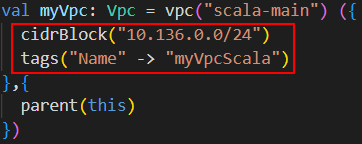
\includegraphics[width=0.5\columnwidth]{case_study/vpc_b_methods} 
%  \captionof{figure}{vpc methods}
%\end{center}\mbox{}\\
Once the enclosing lambda will be invoked inside the \texttt{vpc} function, these methods will be executed, but on which builder?\\
We already mentioned the fact that inside the \texttt{vpc} function a \textit{context} instance of the \texttt{VpcArgs.Builder} is initialized and the \texttt{init} lambda is able to use it as input parameter thanks to the '\texttt{?=>}' operator.
But how can the actual \texttt{cidrBlock} and \texttt{tags} methods know on which builder they are being invoked?\\
We shall consider that those two methods are not the plain Pulumi's Java APIs, but are my own \textit{sugarized} Scala versions of such methods. 
And without surprise, those functions take the \texttt{VpcArgs.Builder} builder as an implicit parameter with the \texttt{using} keyword.\\
This is the signature for the \texttt{cidrBlock} method in the \textit{syntactic sugar} file named "PulumiBuilderUtilFunctionsForScala.scala":\\
\begin{minipage}{\linewidth}
\begin{lstlisting}[numbers=left, numberstyle=\tiny, numbersep=-5pt, stepnumber=1, linewidth=420pt]
  def cidrBlock(param: String | Output[String]) (using b: cidrBlockOwners): Unit
\end{lstlisting}
\end{minipage}
We can notice that we have once again a curried function.
Anyway, from how we have seen before, the \texttt{cidrBlock}, and this holds for all the other builder methods, is called with just a single set of parentheses.
This is due to the fact that the second parentheses here are taking an implicit parameter, properly marked with the \texttt{using} keyword.\\
The \texttt{param} parameter is, as we have seen in the \hyperref[sssec:union]{Union type} paragraph, a union type.
The \texttt{String | Output[String]} type is defined so since the Pulumi Java APIs for the builders' methods accept either a \texttt{String} or an \texttt{Output[String]}.
Actually, in the Java implementation multiple overloaded methods are given since the union type of Scala is not available.\\
The second parentheses are taking an implicit parameter \texttt{b} of the type \texttt{cidrBlockOwners}, that is defined as follows:\\
\begin{minipage}{\linewidth}
\begin{lstlisting}[numbers=left, numberstyle=\tiny, numbersep=-5pt, stepnumber=1, linewidth=420pt]
  type cidrBlockOwners = RouteTableRouteArgs.Builder | SubnetArgs.Builder | VpcArgs.Builder
\end{lstlisting}
\end{minipage}
This is a user defined type that I defined to match the builders of all the \texttt{Args} classes that are interested in having such a \texttt{cidrBlock} parameter to be assigned on their builder instance.
In fact in the Java APIs of Pulumi we have many different \texttt{Args} classes' builders that want to assign the same parameter (aka. \texttt{cidrBlock}) to their own builder.\\
I remind that in the AWS EC2 module there are much more builders of the \texttt{Args} classes that define a \texttt{cidrBlock} method, but my \textit{syntactic sugar} has created the methods for only the classes that I used in the case study.
This choice has been made also for simplicity in presenting the work done, otherwise the \texttt{cidrBlockOwners} type would have been featuring many tens of types.
The fact I used a union type to define this function has two main motivations.
The first is a Scala language constraint that I came across.
Let's say that we wanted to define a function to assign the CIDR block working exclusively for \texttt{VpcArgs.Builder} class.
A definition of such a function would look like:\\
\begin{minipage}{\linewidth}
\begin{lstlisting}[numbers=left, numberstyle=\tiny, numbersep=-5pt, stepnumber=1, linewidth=420pt]
  def cidrBlock(param: String | Output[String]) (using b: VpcArgs.Builder): Unit =
      param match
        case x: String => builder.cidrBlock(x)
        case x: Output[String] => builder.cidrBlock(x)
\end{lstlisting}
\end{minipage}
And now let's define another function that is working for the \texttt{RouteTableRouteArgs.Builder}:\\
\begin{minipage}{\linewidth}
\begin{lstlisting}[numbers=left, numberstyle=\tiny, numbersep=-5pt, stepnumber=1, linewidth=420pt]
  def cidrBlock(param: String | Output[String]) (using b: RouteTableRouteArgs.Builder): Unit =
      param match
        case x: String => builder.cidrBlock(x)
        case x: Output[String] => builder.cidrBlock(x)
\end{lstlisting}
\end{minipage}
First, we can notice that they are actually the same, except for the signature, but such a solution is not going to compile if we try to call the method \texttt{cidrBlock("10.136.0.0/24")} here:\\
\begin{minipage}{\linewidth}
\begin{lstlisting}[numbers=left, numberstyle=\tiny, numbersep=-5pt, stepnumber=1, linewidth=420pt]
  val myVpc: Vpc = vpc("scala-main") ({
    cidrBlock("10.136.0.0/24") \\ ERROR
    tags("Name" -> "myVpcScala")
  },{
    parent(this)
  })
\end{lstlisting}
\end{minipage}
The compiler will tell us that an ambiguous function call is present at the line 2 of this block of code.
This is due to the fact that the functions we defined are curried and their types are \texttt{(String | Output[String]) => (VpcArgs.Builder => Unit)} and \texttt{(String | Output[String]) => (RouteTableRouteArgs.Builder => Unit)} respectively.
When we call \texttt{cidrBlock("10.136.0.0/24")} on the line 2 of the code showed above, we are partially applying the curried function and so the compiler doesn't know which function we are trying to call, since it can't infer the exact function call basing only on a different return type (that is the only difference in the two returned partially applied functions).\\
The second reason is that our \textit{all-in-one} solution is reducing the size of the generated \textit{sugared} code, since we have just one single method instead of having as many as the builders of the \texttt{Args} classes that require that methods are.\\

Now we are ready to present the entire \texttt{cidrBlock} method:\\
\begin{minipage}{\linewidth}
\begin{lstlisting}[numbers=left, numberstyle=\tiny, numbersep=-5pt, stepnumber=1, linewidth=420pt]
  def cidrBlock(param: String | Output[String]) (using b: cidrBlockOwners): Unit =
    b match
      case builder: RouteTableRouteArgs.Builder =>
        param match
          case x: String => builder.cidrBlock(x)
          case x: Output[String] => builder.cidrBlock(x)
      case builder: SubnetArgs.Builder =>
        param match
          case x: String => builder.cidrBlock(x)
          case x: Output[String] => builder.cidrBlock(x)
      case builder: VpcArgs.Builder =>
        param match
          case x: String => builder.cidrBlock(x)
          case x: Output[String] => builder.cidrBlock(x)
\end{lstlisting}
\end{minipage}
The body of the function is quite simple in its functioning.
It uses the pattern matching to match the correct builder type and then uses pattern matching once more to match the \texttt{param} parameter to a \texttt{String} or an \texttt{Ouput[String]}.
Finally it calls the Java API of Pulumi to set the \texttt{cidrBlock} parameter on the builder instance \texttt{b}.\\
The fact we have duplicated code here is inevitable.
This is the only solution since if we try to split the duplicated code into a helper function, we would fall again in the 'ambiguous call' compiler error presented above.
But since this is automatically generated code, it is not a real problem to have some duplicated code.\\
\newline
To have the final picture of all the functioning let's consider this image:
\begin{center}
  \hspace*{-3cm}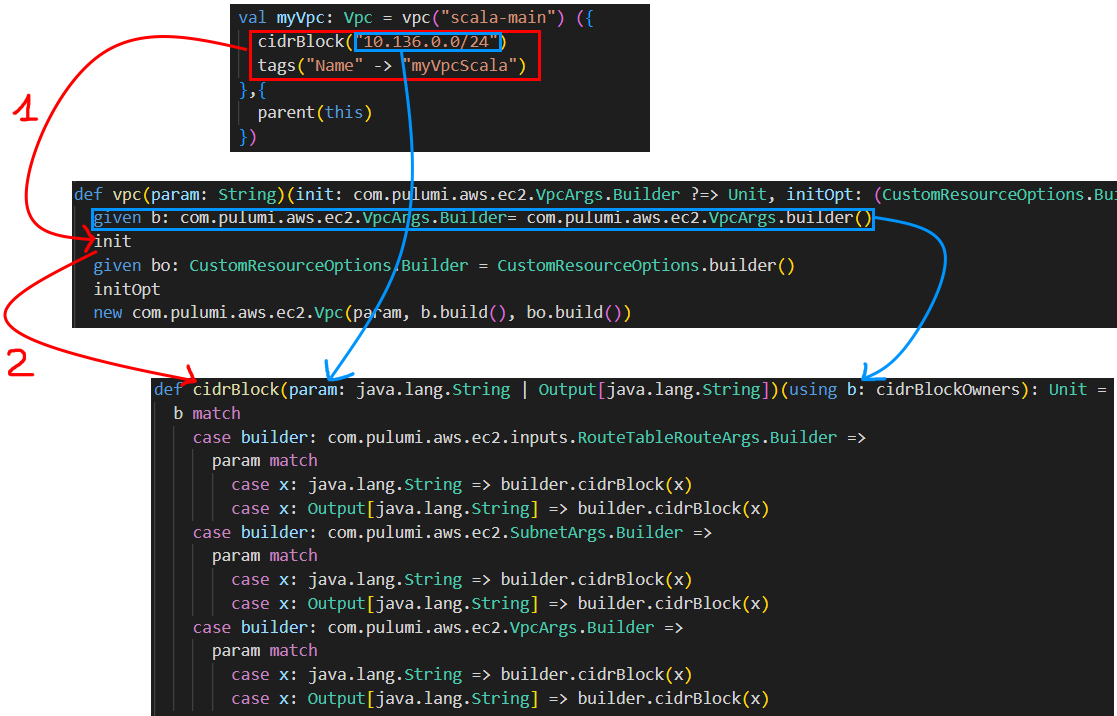
\includegraphics[width=1.4\columnwidth]{case_study/syn-sug-flow} 
  \captionof{figure}{Function calls flow and parameters passing for the VPC declaration}
\end{center}\mbox{}\\
We can see how the lambda with the calls to our defined methods \texttt{cidrBlock} and \texttt{tags} is passed as the \text{init} parameter of the \textit{sugared} \texttt{vpc} function.
Inside the \texttt{vpc} function we execute that lambda and so, the \texttt{cidrBlock} method is invoked.\\
In blue we can see from where the parameters of the \texttt{cidrBlock} method are coming from.
The \texttt{String} representing the CIDR block is coming directly from the explicit parameter that we passed,
while the \texttt{VpcArgs} builder is implicitly injected from the compiler since a \textit{given} instance is defined inside the \texttt{vpc} function and the \texttt{b} parameter of the \texttt{cidrBlock} method is marked with \texttt{using}.

\subsubsection{Implicit conversion functions}
\label{sssec:implicit-converion-functions}
On top of this, to boost our \textit{syntactic sugar} I defined also two extra functions: \texttt{tupleToMap} and \texttt{elemToList}.
The purpose of these functions is to achieve the tricks that I mentioned previously (in the \hyperref[sssec:vpc-creation-scala]{Vpc creation in Scala} and in the \hyperref[sssec:routetable-creation-scala]{Routetable creation in Scala}) about not needing to explicitly instantiate a singleton \texttt{Map} and a singleton \texttt{List} while passing a single argument to the \texttt{tags} or the \texttt{routes} methods.
The \texttt{tupleToMap} function is implemented like this:\\
\begin{minipage}{\linewidth}
\begin{lstlisting}[numbers=left, numberstyle=\tiny, numbersep=-5pt, stepnumber=1, linewidth=420pt]
  given tupleToMap[A, B]: Conversion[(A, B), Map[A, B]] =
	  (tuple: (A, B)) => Map(tuple)
\end{lstlisting}
\end{minipage}
We can notice that the function that converts our \texttt{tuple} into a singleton \texttt{Map} is based on the \texttt{Converion} class of Scala.
When a suitable argument for the conversion of type \texttt{(A, B)} is found in the code, and a \texttt{Map[A, B]} type is expected, then the compiler will apply the conversion to that type.
This is exactly what happens with our \texttt{tuple} as a single parameter passed to the \texttt{tags} method.\\
The \texttt{elemToList} function is defined in this way instead:\\
\begin{minipage}{\linewidth}
\begin{lstlisting}[numbers=left, numberstyle=\tiny, numbersep=-5pt, stepnumber=1, linewidth=420pt]
  given elemToList[A <: ResourceArgs]: Conversion[A, List[A]] =
	  (elem: A) => List(elem)
\end{lstlisting}
\end{minipage}
The functioning is analogous to \texttt{tupleToMap}, but here we added the extra constraint that \texttt{A} must be a subtype of the \texttt{ResourceArgs} type.
This will prevent too generic undesired conversions that could create problems in the compilation of our program.

\subsection{Functor and Monad implementation for the Output type}
After having introduced the concept of functor and monad in the \hyperref[sssec:functors-monads]{Functors and monads} section, it is here shown how the implementation of the monad for the \texttt{Ouput} type has been achieved.\\
Since a monad is also a functor, let's see how \texttt{Functor[Output]} has been implemented.

\subsubsection{Functor implementation}
First a \texttt{Functor} trait has been defined:\\
\begin{minipage}{\linewidth}
\begin{lstlisting}[numbers=left, numberstyle=\tiny, numbersep=-5pt, stepnumber=1, linewidth=420pt]
  trait Functor[F[_]]:
    extension [A](x: F[A])
      def map[B](f: A => B): F[B]
\end{lstlisting}
\end{minipage}
A type \texttt{Output} to be a functor has to implement a \texttt{map} method, that as we have already seen is provided as an extension method.\\
The functor for the \texttt{Output} type is implemented like this:\\
\begin{minipage}{\linewidth}
\begin{lstlisting}[numbers=left, numberstyle=\tiny, numbersep=-5pt, stepnumber=1, linewidth=420pt]
  given Functor[Output] with
    extension [A](oa: Output[A])
      def map[B](f: A => B): Output[B] =
        oa.applyValue(f.asJava)
\end{lstlisting}
\end{minipage}
The implementation of the \texttt{map} method relies on the Java APIs of Pulumi, where the \texttt{applyValue} method from the Output class is provided.\\
The signature of the given method is:
\begin{verbatim}
  default <U> Output<U> applyValue(Function<T, U> func)
\end{verbatim}
We are interested in observing that this method takes a function that transforms a value of a type \texttt{T} in a value of type \texttt{U}, and then it returns an \texttt{Output[U]} value as result.
This signature is exactly the same of the one of our \texttt{map} method.\\
In fact it is sufficient to pass the function \texttt{f} taken in input from the \texttt{map} function and pass it directly to \texttt{applyValue}.
To be precise, being \texttt{applyValue} a Java function that expects another Java fucntion as input parameter, we have to first convert our Scala function \texttt{f} to a Java function.
We achieve this by using the \texttt{.asJava} method from the \texttt{scala.jdk.FunctionConverters.\_} conversion library for Scala.

\subsubsection{Monad implementation}
As for the \texttt{Functor}, the \texttt{Monad} trait has been defined:\\
\begin{minipage}{\linewidth}
\begin{lstlisting}[numbers=left, numberstyle=\tiny, numbersep=-5pt, stepnumber=1, linewidth=420pt]
  trait Monad[F[_]] extends Functor[F]:
    // The unit value for a monad
    def pure[A](x: A): F[A]

    extension [A](x: F[A])
      // The fundamental composition operation
      def flatMap[B](f: A => F[B]): F[B]
      // The `map` operation can now be defined in terms of `flatMap`
      def map[B](f: A => B) = x.flatMap(f.andThen(pure))
\end{lstlisting}
\end{minipage}
A monad, to be called so, must define a \texttt{pure} function.
I remind that such a method puts a value inside a \textit{context}.\\
Then the \texttt{faltMap}, that is the other method required from a monad, is defined as an extension method.\\
The \texttt{map} method can now be redefined using \texttt{flatMap}.
This is letting us not depend any more on the \texttt{.applyValue} from the Pulumi libraries for Java, because we can now use \texttt{flatMap} to achieve the desired result.\\
The monad for the \texttt{Output} type is implemented in this way:\\
\begin{minipage}{\linewidth}
\begin{lstlisting}[numbers=left, numberstyle=\tiny, numbersep=-5pt, stepnumber=1, linewidth=420pt]
  given Monad[Output] with
    def pure[A](x: A): Output[A] = Output.of(x)
    extension [A](oa: Output[A])
      def flatMap[B](f: A => Output[B]): Output[B] = oa.apply(f.asJava)
\end{lstlisting}
\end{minipage}
The pure method is defined with the Java's Pulumi method \texttt{of}.
It simply boxes the value in an \texttt{Output} \textit{context}.\\
The \texttt{flatMap} function for the \texttt{Output[A]} type is implemented using the \texttt{.apply} function offered from the Pulumi's Java Output class.
The \texttt{apply} function has a different type from the \texttt{applyValue} one.
As we have seen above, \texttt{applyValue} is matching with the type of \texttt{map}, while the \texttt{apply} has the following signature:
\begin{verbatim}
  <U> Output<U> apply(Function<T, Output<U>> func)
\end{verbatim}
Since the function passed to \texttt{apply} takes a type \texttt{T} as input and returns a type \texttt{Output<U>} as result, and the whole \texttt{apply} returns an \texttt{Output<U>}, we have a perfect type match with the \texttt{flatMap} signature.
In fact it will suffice us to use \texttt{apply.(f.asSJava)} to get the work done.\\
Thanks to this implementation we are able, as we have seen in the \hyperref[sssec:subnets-creation]{Subnets creation in Scala} paragraph, 
to use \texttt{map} inside the for yield construct to \textit{unbox} the inner values of the \texttt{Output} types and achieve the desired results.
%In fact, \texttt{availabilityZonesNames()} is Output[GetAvailabilityZonesResult], and being now Output a monad, the map function is supported.
With all this, we succeeded in both getting rid of the \texttt{.pulumiall} method while having an even more readable and expressive syntax.

\subsection{Automatic code generation for the \textit{syntactic sugar}}
The generation of the \textit{syntactic sugar} code required the following 2 passages:
\begin{itemize}
  \item Analyze the source code of Pulumi's Java APIs for AWS EC2 in order to infer some information about their structure. To be precise, we want to understand which resources constructors and which builders' methods are present% in the Builder of each \texttt{Args} class
  \item Use the extracted information to automatically generate the \textit{sugared} code for the PulumiUtilFunctionsForScala.scala and PulumiBuilderUtilFunctionsForScala.scala files
\end{itemize}
The first step has been quite straight forward with the aid of the JavaParser library.
The second step has been more problematic.\\
I'll introduce now the failed approaches for the second step and, in the next section, the details about the final solutions will be presented.

\subsubsection{Scala 3 \textit{macro}s}
As a first attempt for the automatic generation of the \textit{syntactic sugar}, I tried to use the metaprogramming features offered from the new Scala 3 \textit{macro}s to represent the autogenerated code in the form of an \gls{abstract syntax tree} (AST).
This solution was potentially promising, since Scala also offers the opportunity to convert these ASTs in code and vice versa at compile time, and so telling us about any error at compile time.
The problem encountered was that once we defined the \textit{macro} for a new type (like the \texttt{cidrBlockOwners} union type), such a type wasn't available at compile time for the other code.
In other words, the types generated through the \textit{macro}, can't be referenced in the same project since the whole compilation must be finished before having the chance to use the brand-new types.\\
I'll report here the work done, that is the attempt to define a custom type to be later used in the same project.
In particular, the type definition was trying to address the generation of the custom types, like \texttt{cidrBlockOwners}. 
These types were to be used later, in the same project, with other \textit{macro}s that would have represented the builders' methods and the constructors for the resources.

\paragraph{What is a \textit{macro}}
Thanks to the useful introduction provided by Pawel L. on \href{https://medium.com/codex/scala-3-macros-without-pain-ce54d116880a}{Medium}, I'll report here the key concepts of the Scala 3 \textit{macro}s.
A Scala 3 \textit{macro} is a piece of code \textbf{executed by the compiler}.
With the \textit{macro}s, it is possible to analyze and generate code.
If an expression of type \texttt{T} should be used by the \textit{macro}, it needs to be converted to \texttt{Expr[T]} — the representation suitable for the \textit{macro}.
This process is called \textit{quotation}.
The code representation created in the \textit{macro} is converted back and embedded in the program in the process of \textit{splicing}.\\
Scala 3 \textit{macro}s manage the code as an AST. To be precise the Scala 3 implementation of the AST is used, that is called Typed Abstract Syntax Tree (TASTy).\\
A \textit{macro} in general is defined by two functions.
One is used to call the \textit{macro} in the code and the other is used define its implementation.\\
Now let's consider a \textit{macro} to define a new type with a custom name that represents the \texttt{String | Boolean} union type.
The function that implements the \textit{macro} is the following one:\\
\begin{minipage}{\linewidth}
  \begin{lstlisting}[numbers=left, numberstyle=\tiny, numbersep=-5pt, stepnumber=1]
    def defineNewTypeImpl(name: Expr[String], types:
         Expr[Seq[String]])(using ctx: Quotes) : Expr[Any] = 
      '{ type $name = String | Boolean }
  \end{lstlisting}
\end{minipage}
The \textit{quoting}, identified by the \texttt{'\{...\}} syntax, is encapsulating the code contained within the curly brackets in a TASTy representation.
We can also note the \texttt{\$name} syntax within the curly brackets.
In fact, since the \texttt{name} parameter is of type \texttt{Expr}, and hence is represented as a TASTy, we have to convert it to code in order to use it inside the curly brackets along with the rest of the code.
To achieve this we used the splicing: \texttt{\$}.\\
Now let's consider instead the function that we'll use to call the \textit{macro}:\\
\begin{minipage}{\linewidth}
  \begin{lstlisting}[numbers=left, numberstyle=\tiny, numbersep=-5pt, stepnumber=1]
    inline def defineNewType(inline name: String, inline types: String*): Any = 
      ${ TypeGenMacroImpl.defineNewTypeImpl('name, 'types) }
  \end{lstlisting}
\end{minipage}
The first thing we can notice from such a function is the presence of the \texttt{inline} keyword.
The \textit{inlining}, in Scala, is the replacement of the code in the place of the usage instead of its reference.\\
So when we'll call this function, its body will be replaced by the compiler at the site of the function call.
Since the body of this function is the \textit{splicing} of the call to the \textit{macro} implementation, the code that will is going to be replaced will be, in truth, the one returned by the definition of the \textit{macro}.\\
We evince that the key to work with \textit{macro}s is the combo between the \textit{inlining} and the \textit{quoting}/\textit{splicing}.
As a final result we'll have the compilation of the code defined within the body of the \textit{macro} implementation in the place of the \textit{macro} call.\\
%The final result will be the compilation of a code that has the body of the definition of the \textit{macro} in place of the function call.\\
\newline
What I wanted to achieve with all this was the possibility to define a new type through a \textit{macro} and reference that type somewhere else in the project.
So I created this object for the definition of a new type:\\
\begin{minipage}{\linewidth}
  \begin{lstlisting}[numbers=left, numberstyle=\tiny, numbersep=-5pt, stepnumber=1]
    object NewTypeDefinition {
      defineNewType("MyType", "")
    }
  \end{lstlisting}
\end{minipage}
With this code we are actually asking the compiler to replace the code of the \texttt{defineNewTypeImpl} \textit{macro} function, with \texttt{"MyType"} as input parameter in place of the function call at line 2 of the block of code just presented.\\
The next step was to reference the newly created type somewhere else in the code, in this way:\\
\begin{minipage}{\linewidth}
  \begin{lstlisting}[numbers=left, numberstyle=\tiny, numbersep=-5pt, stepnumber=1]
    @main def hello: Unit = 
      val x: MyType = "MyString value" \\ comp. error
  \end{lstlisting}
\end{minipage}
Sadly this is not possible because of the problem that has been explained at the beginning of this section.
The \texttt{MyType} type generated through the \textit{macro} is not available for us until the compilation of the whole project is complete.
Hence, where we are trying to define the value \texttt{x} of type \texttt{MyType}, the compiler complains with the error "\texttt{Not found: type MyType}".\\
This problem caused the whole \textit{macro} approach to fail.


\subsubsection{Scalameta}
Another option was represented by Scalameta: a library to read, analyze, transform and generate Scala programs.
Sadly, it isn't compatible with Scala 3, and so I had no chance to use it.
If the support for Scala 3 will be added to Scalameta, it should be considered a better approach for the generation of the \textit{syntactic sugar} code in the future.

\subsubsection{A naïve approach as solution}
In the end, for the second step, a standard \textit{naïve} approach has been adopted.
The auto-generated code is created with a program that inserts the piece of information extracted from the analysis of the Java APIs into a template for the PulumiBuilderUtilFunctionsForScala.scala and the PulumiUtilFunctionsForScala.scala files.
The generated code can then be exported as a library and included into the dependencies of the building system used in the Pulumi Scala project.

\subsection{Pulumi Java APIs libraries inspection with JavaParser}
Since the code of the project for the inspection is quite verbose (JavaParser is a Java library) and not particularly interesting for the final objective of the thesis, I won't report any code here.
I'll limit to describe the steps that are done to infer the required information from the Java libraries for Pulumi.

\subsubsection{Non Args and Args classes}
In the Java APIs of Pulumi we have two kind of files (and so classes).
The firsts are the \textbf{non} ...\texttt{Args} files, that are those files that contain the API for the constructors of a given resource.
The second kind of files are represented by the \texttt{Args} files.
These classes contain the \texttt{Builder} definition of the respective class and the APIs of the respective builder methods. % used to pass the arguments of the resource while building it with an instance of a builder.
For example, we have the Vpc.java file and the VpcArgs.java files.

\subsubsection{DirExplorer}
The first class that I defined is \texttt{DirExplorer}. This class has the objective to find all the files in a given directory (and the files in the subdirectories), letting us apply some extra logic during its traverse.
We'll be using such a class in a \texttt{InferInformation} class to extract all the names of the files of our interest.\\

\subsubsection{InferInformation}
In the \texttt{InferInformation} class we have 3 methods:
\begin{description}
  \item[listBuilderMethods] is the function that opens every ...\texttt{Args.java} file and, after having parsed an AST of such file, will save all the methods of its builder in a data structure that we'll introduce soon
  \item[listConstructorMethods] is the function that opens every \textbf{non} ...\texttt{Args.java} and, after having parsed the corresponding AST, checks if a public constructor for the given resource is available. In such a case it will add the name of the class to a List that represents all the constructors that should be generated for our \textit{syntactic sugar} code
  \item[listFiles] is an helper function for the other two methods that just provides the file names of the classes inspected
\end{description}
The data structure used to store the builders' method has the type \texttt{Map[String, (String, LinkedList[String])]}.
The key of this \texttt{Map} is the name of every different builder method encountered during the parsing of the files.
The value of the \texttt{Map} is a list of all the ...\texttt{Args} classes that contain such a method.
In other worlds, for each method we map all the classes that define such a function.
The entry for the \texttt{cidrBlock} method on the \texttt{Map} (parsing all the AWS EC2 Java files) looks like this:
\begin{verbatim}
cidrBlock: [
  DefaultNetworkAclEgressArgs,
  DefaultNetworkAclIngressArgs,
  DefaultRouteTableRouteArgs,
  GetSubnetArgs,
  GetSubnetPlainArgs,
  GetVpcArgs,
  GetVpcPeeringConnectionArgs,
  GetVpcPeeringConnectionPlainArgs,
  GetVpcPlainArgs,
  NetworkAclEgressArgs,
  NetworkAclIngressArgs,
  RouteTableRouteArgs,
  NetworkAclRuleArgs,
  SubnetArgs,
  SubnetCidrReservationArgs,
  VpcArgs,
  VpcIpv4CidrBlockAssociationArgs
]
\end{verbatim}
Among all this values, we can find the \texttt{VpcArgs}, \texttt{RouteTableRouteArgs} and \texttt{SubnetArgs} that we used in our implementation, and to which we passed a CIDR block using the \texttt{cidrBlock} method.\\
With the information achieved we are now ready to fill in the templates and generate the \textit{syntactic sugar} for the Scala APIs of Pulumi.

\subsection{Raw automatic \textit{syntactic sugar} code generation}
The class that generates all the code is quite simple.
A Java \texttt{FileWriter} will take care of writing all the strings that represent our code in the PulumiBuilderUtilFunctionsForScala.scala and PulumiUtilFunctionsForScala.scala files.\\
We have two functions, named \texttt{writeContentForBuilders} and \texttt{writeContentForConstructors} that will write all the \textit{various pieces} of generated code into the files using the \texttt{FileWriter}.
With \textit{various pieces} I refer to the generated types for the methods of the builders, the imports, the conversion functions, etc.\\
Finally we have a bunch of functions that fill the various templates to generate the \textit{various pieces} of code.
These functions are: \texttt{generateTypes}, \texttt{generateBuilderMethods}, \texttt{generateConstructors}, and \texttt{generateImplicitConversionFunctions}.
To have an idea of how the filling of a template works let's consider the \texttt{generateConstructors} function:\\
%\begin{minipage}{\linewidth}
%  \begin{lstlisting}[numbers=left, numberstyle=\tiny, numbersep=-5pt, stepnumber=1]
%  def generateConstructors(extractedConstructors: Array[String]) : Array[String] =
%    for con <- extractedConstructors
%      yield {
%        val functionName = con.drop(con.lastIndexOf('.') + 1)
%        val builderCon = con + "Args.Builder";
%        "def " + functionName.head.toLower + functionName.tail +
%          "(param: String)(init: " +
%          builderCon +
%          " ?=> Unit, initOpt: (CustomResourceOptions.Builder ?=> Unit) = baseOpts): " +
%          con + " =\n" +
%        "\tgiven b: " + builderCon + "= " + con + "Args.builder()\n" +
%        "\tinit\n" +
%        "\tgiven bo: CustomResourceOptions.Builder = CustomResourceOptions.builder()\n" +
%        "\tinitOpt\n" +
%        "\tnew " + con + "(param, b.build(), bo.build())"
%      }
%  \end{lstlisting}
% \end{minipage}
\begin{center}
  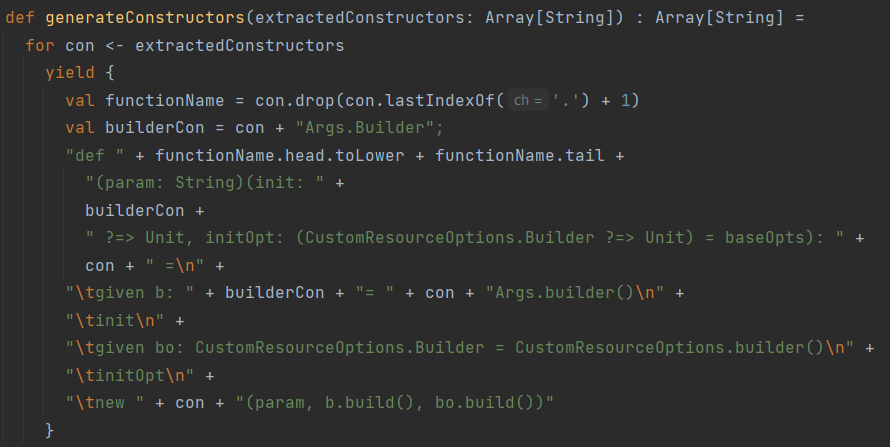
\includegraphics[width=1\columnwidth]{case_study/template_gen} 
  \captionof{figure}{Code for automatic generation of the resources constructors}
\end{center}\mbox{}\\
The template is filled with the variables that represent the name of the constructors, and this is done for each constructor that has been found.\\
Since also the other functions are similar to this one, they won't be reported here.

\subsection{The automatically generated \textit{syntactic sugar} code}
Since the generated files contain many hundreds of lines of code, I'll report here only some samples of each file.\\

\subsubsection{PulumiBuilderUtilFunctionsForScala}
First we have some default imports:\\
\begin{minipage}{\linewidth}
  \begin{lstlisting}[numbers=left, numberstyle=\tiny, numbersep=-5pt, stepnumber=1]
    package com.cisotto.myvpc.builder

    import com.pulumi.Context
    import com.pulumi.Pulumi
    import com.pulumi.core.Output
    import com.pulumi.resources.{CustomResourceOptions, Resource}
    import scala.collection.JavaConverters._
    import collection.convert.ImplicitConversionsToScala.`collection AsScalaIterable`
    import scala.compiletime.ops.boolean
    import scala.compiletime.ops.string
    import scala.language.implicitConversions
    import com.pulumi.resources.CustomResourceOptions
    import com.pulumi.resources.ResourceArgs
  \end{lstlisting}
 \end{minipage}
%\begin{center}
%  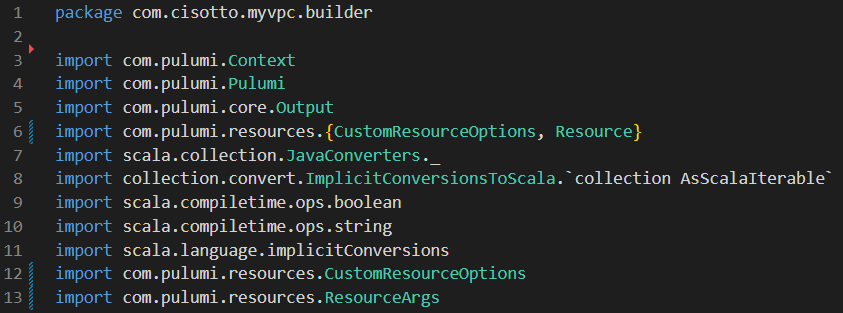
\includegraphics[width=1\columnwidth]{case_study/build_imports} 
%  \captionof{figure}{Default import}
%\end{center}\mbox{}\\
Then, we have all the generated union types, that look like this:\\
\begin{minipage}{\linewidth}
  \begin{lstlisting}[numbers=left, numberstyle=\tiny, numbersep=-5pt, stepnumber=1]
    ...
    type vpcIdOwners = InternetGatewayArgs.Builder | RouteTableArgs.Builder | SubnetArgs.Builder
    type gatewayIdOwners = RouteTableRouteArgs.Builder | RouteTableAssociationArgs.Builder
    type localGatewayIdOwners = RouteTableRouteArgs.Builder
    type tagsOwners = InternetGatewayArgs.Builder | RouteTableArgs.Builder | ubnetArgs.Builder | VpcArgs.Builder
    ...
  \end{lstlisting}
 \end{minipage}
%\begin{center}
%  \hspace*{-3cm}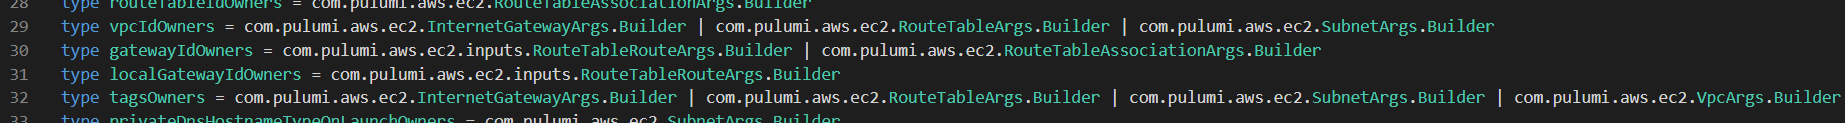
\includegraphics[width=1.5\columnwidth]{case_study/generated_union_types} 
%  \captionof{figure}{Generated union types}
%\end{center}\mbox{}\\
The implicit conversion functions are then printed:\\
\begin{minipage}{\linewidth}
  \begin{lstlisting}[numbers=left, numberstyle=\tiny, numbersep=-5pt, stepnumber=1]
    given tupleToMap[A, B]: Conversion[(A, B), Map[A, B]] =
      (tuple: (A, B)) => Map(tuple)
  
    given elemToList[A <: ResourceArgs]: Conversion[A, List[A]] =
      (elem: A) => List(elem)
  \end{lstlisting}
 \end{minipage}
%\begin{center}
%  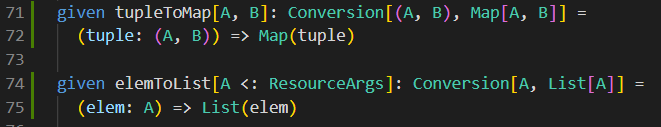
\includegraphics[width=1\columnwidth]{case_study/implicit_conv_fun} 
%  \captionof{figure}{Implicit conversion functions}
%\end{center}\mbox{}\\
Finally, we have all the builders' methods that we encountered during our visit of the files with the JavaParser project:\\
  \begin{lstlisting}[numbers=left, numberstyle=\tiny, numbersep=-5pt, stepnumber=1]
  ...
  def egressOnlyGatewayId(param: String | Output[String])(using b: egressOnlyGatewayIdOwners): Unit =
    b match
      case builder: RouteTableRouteArgs.Builder =>
        param match
          case x: String => builder.egressOnlyGatewayId(x)
          case x: Output[String] => builder.egressOnlyGatewayId(x)
  
  
  def ipv6IpamPoolId(param: String | Output[String])(using b: ipv6IpamPoolIdOwners): Unit =
    b match
      case builder: VpcArgs.Builder =>
        param match
          case x: String => builder.ipv6IpamPoolId(x)
          case x: Output[String] => builder.ipv6IpamPoolId(x)
  
  
  def cidrBlock(param: String | Output[String])(using b: cidrBlockOwners): Unit =
    b match
      case builder: RouteTableRouteArgs.Builder =>
        param match
          case x: String => builder.cidrBlock(x)
          case x: Output[String] => builder.cidrBlock(x)
      case builder: SubnetArgs.Builder =>
        param match
          case x: String => builder.cidrBlock(x)
          case x: Output[String] => builder.cidrBlock(x)
      case builder: VpcArgs.Builder =>
        param match
          case x: String => builder.cidrBlock(x)
          case x: Output[String] => builder.cidrBlock(x)
  ...
  \end{lstlisting}
%\begin{center}
%  \hspace*{-3cm}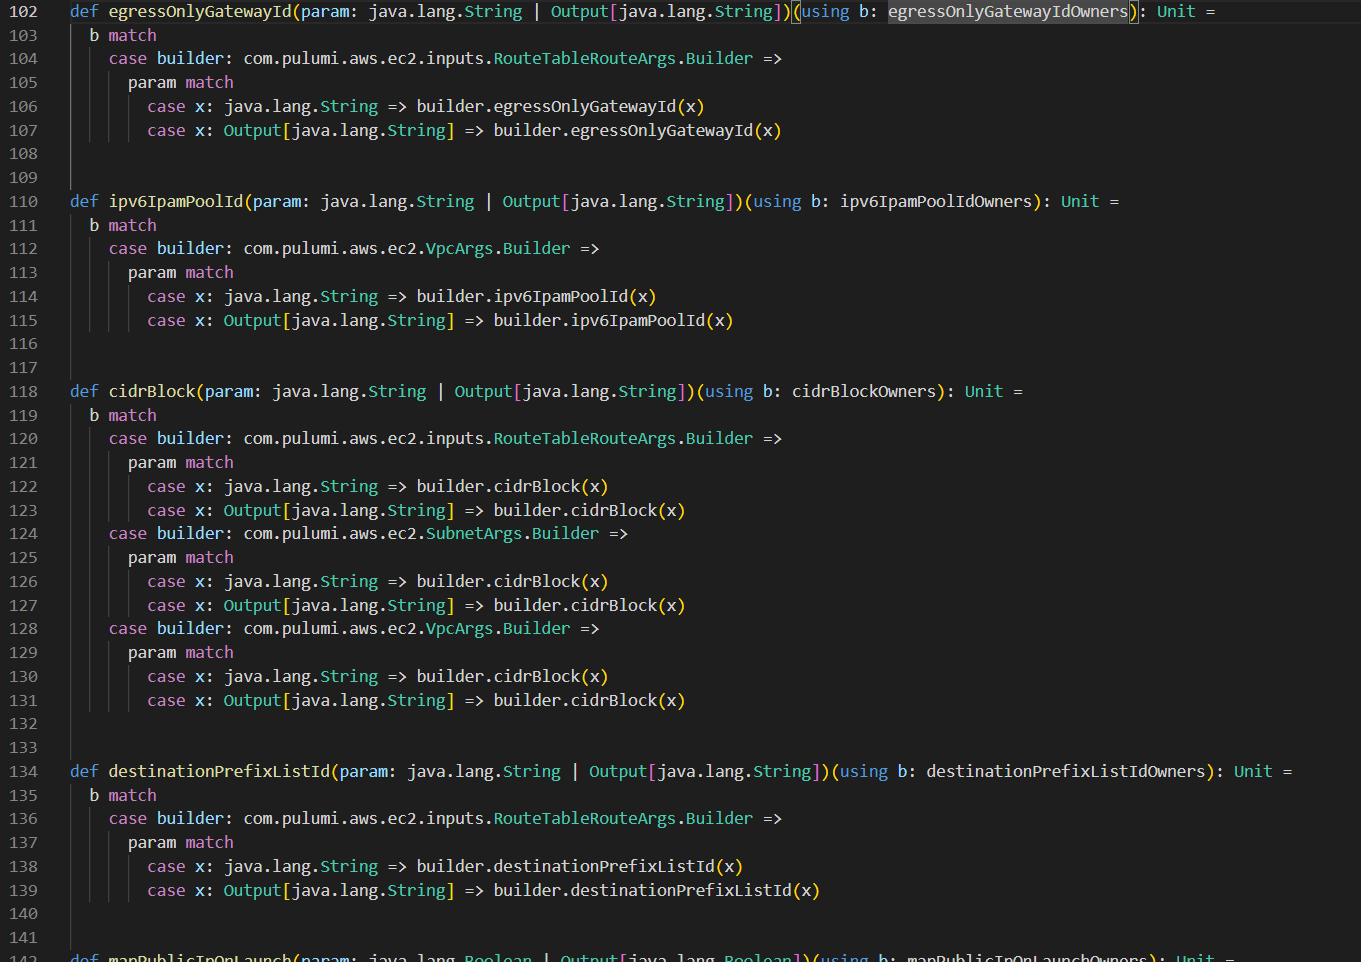
\includegraphics[width=1.4\columnwidth]{case_study/generated_builder_methods} 
%  \captionof{figure}{Generated builders' methods}
%\end{center}\mbox{}\\

\subsubsection{PulumiUtilFunctionsForScala}
Also here we start with some default imports, then we have the \texttt{baseOpts} function and then all the constructors for the various resources.
The constructors look like this:\\
\begin{minipage}{\linewidth}
  \begin{lstlisting}[numbers=left, numberstyle=\tiny, numbersep=-5pt, stepnumber=1]
    def baseOpts(using o: CustomResourceOptions.Builder) : Unit = {} 

    def ami(param: String) (init: AmiArgs.Builder ?=> Unit, 
        initOpt: (CustomResourceOptions.Builder ?=> Unit) = baseOpts): Ami =
      given b = com.pulumi.aws.ec2.AmiArgs.builder()
      init
      given bo = CustomResourceOptions.builder()
      initOpt
      new Ami(param, b.build(), bo.build())
    
    def amiCopy(param: String)(init: AmiCopyArgs.Builder ?=> Unit, 
        initOpt: (CustomResourceOptions.Builder ?=> Unit) = baseOpts): AmiCopy =
      given b = AmiCopyArgs.builder()
      init
      given bo = CustomResourceOptions.builder()
      initOpt
      new AmiCopy(param, b.build(), bo.build())
    
    def amiFromInstance(param: String)(init: AmiFromInstanceArgs.Builder ?=> Unit, 
        initOpt: (CustomResourceOptions.Builder ?=> Unit) = baseOpts): AmiFromInstance =
      given b = AmiFromInstanceArgs.builder()
      init
      given bo = CustomResourceOptions.builder()
      initOpt
      new AmiFromInstance(param, b.build(), bo.build())
  \end{lstlisting}
\end{minipage}

%\begin{center}
%  \hspace*{-3cm}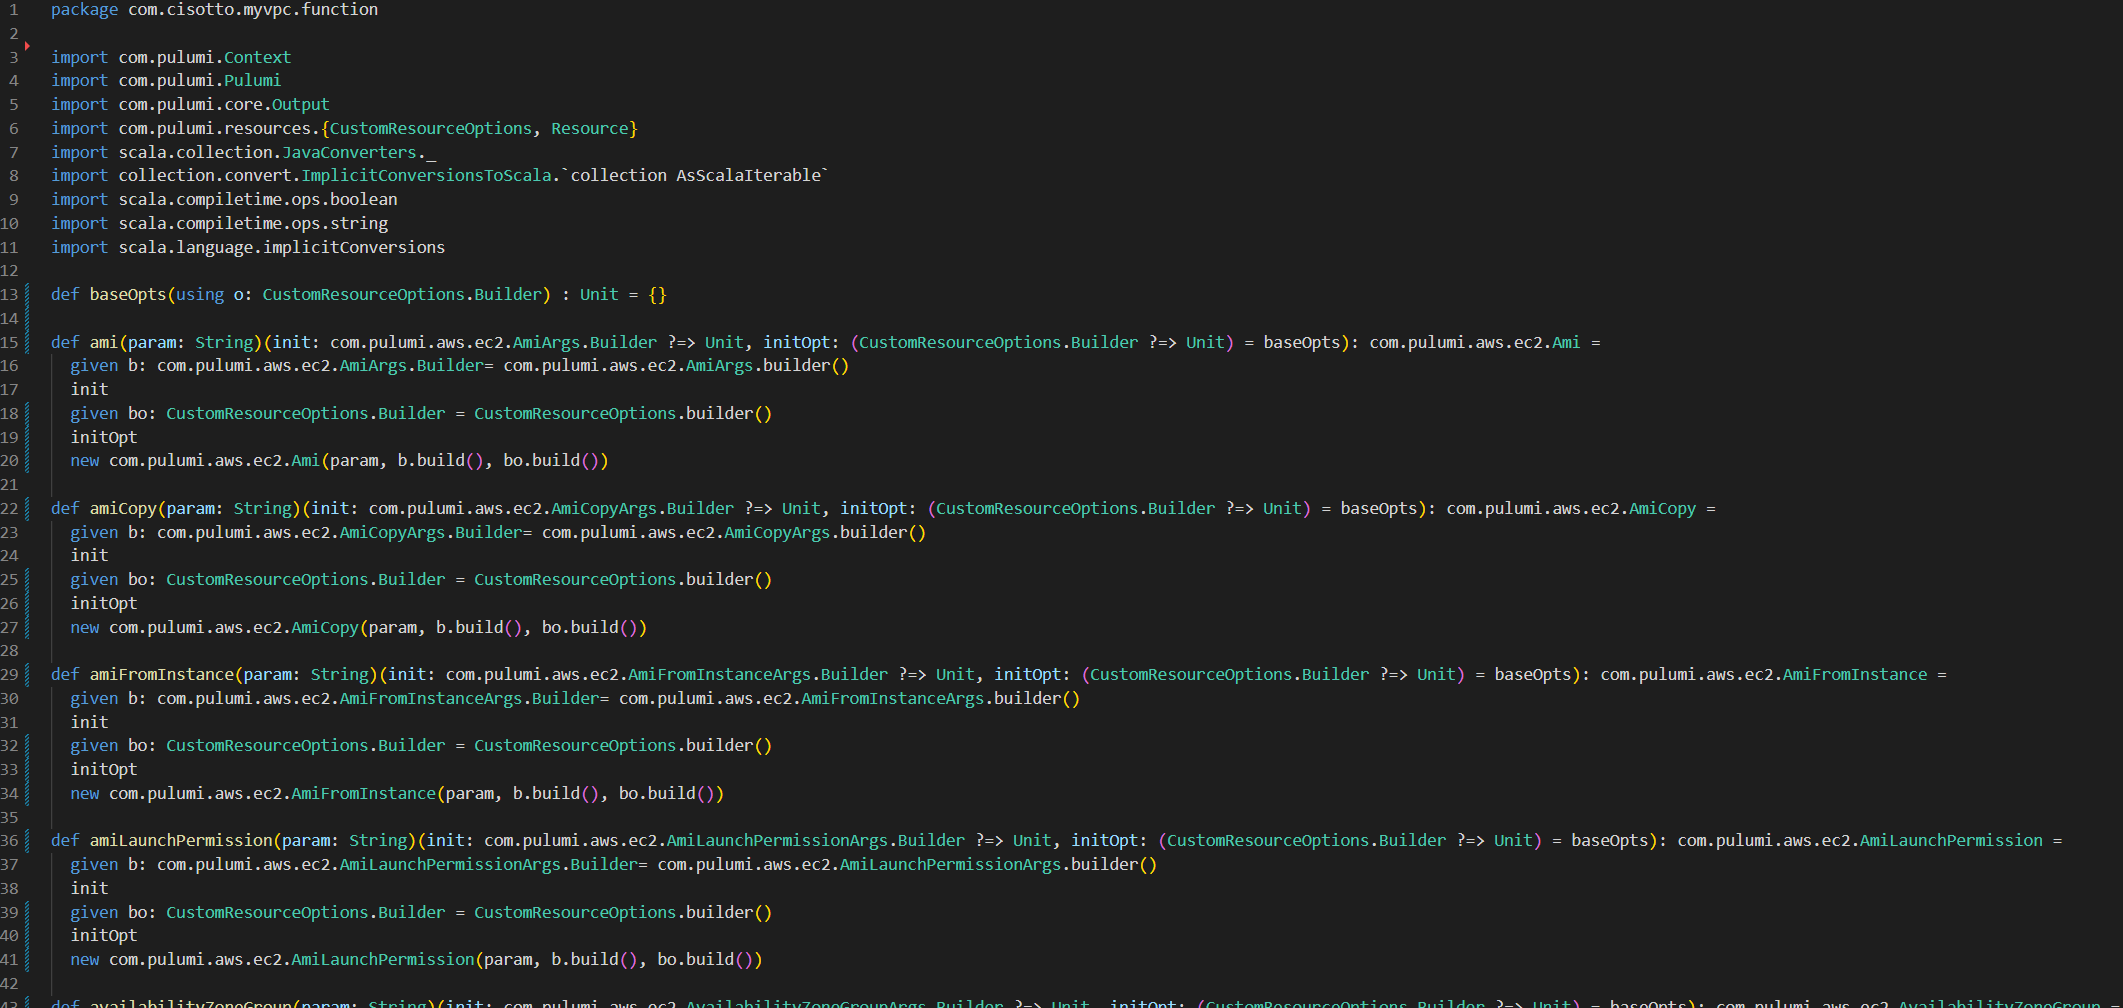
\includegraphics[width=1.4\columnwidth]{case_study/generated_constructors} 
%  \captionof{figure}{baseOpts function and generated constructors}
%\end{center}\mbox{}\\

\subsubsection{Final observations on the generated code}
The builders' methods are really similar to each other, but they are not all following the same exact pattern across the whole AWS EC2 module.
Due to this fact, the generation of the code was affordable for the resources used in the case study, but to cover some corner cases for the rest of the resources some extra work both for the parser and for the algorithm that fills in the template would have been required.
Because of the lack of time and since was not the final aim of the thesis to develop a complete support of Scala for all the AWS EC2 module, only the support for the used resources has been generated.\\
The constructors, instead, are all similar to each other and a complete support for AWS EC2 has been generated.